\begin{frame}\frametitle{$e\rightarrow\gamma$ background estimation. Method Description and Fit Model}
{\footnotesize\bfseries{Method Description}}
\scriptsize
\begin{itemize}
  \item Get $N_{MC-Zpeak}^{e\rightarrow\gamma}$ (number of $e\rightarrow\gamma$ events under the Z-peak based on the MC prediction); done by counting
  \item Get $N_{data-Zpeak}^{e\rightarrow\gamma}$ (number of $e\rightarrow\gamma$ events under the Z-peak from data); done by fitting
  \item Get $N_{MC-nom}^{e\rightarrow\gamma}$ (number of $e\rightarrow\gamma$ events in the nominal range based on the MC prediction); done by counting
  \item Get $N_{data-nom}^{e\rightarrow\gamma}$ (number of $e\rightarrow\gamma$ events in the nominal range based on the MC predictionfrom data); done by scaling {\footnotesize\bfseries{$N_{data-nom}^{e\rightarrow\gamma} = N_{MC-nom}^{e\rightarrow\gamma} \cdot N_{data-Zpeak}^{e\rightarrow\gamma}/N_{MC-Zpeak}^{e\rightarrow\gamma}$}}
\end{itemize}

{\footnotesize\bfseries{Fit Model}}\\
\scriptsize
$N_{sig} \cdot (RooNDKeysPdf~x~Gaussian) +  N_{bkg} \cdot (RooCMSShapePdf)$\\
\end{frame}% end of \frametitle{Fit Model}

\begin{frame}\frametitle{$e\rightarrow\gamma$ background estimation. Fit Binning and Details}
\scriptsize
\begin{itemize}
  \item perform fits separately for each (pt,eta) bin
  \item pt binning is analysis binning
  \item eta binning is 
     \begin{itemize}
        \tiny
        \item 15-20-25-30-35-45-55 GeV
           \begin{itemize}
              \tiny
              \item barrel: 0.00-0.10-0.50-1.00-1.44
              \item endcap: 1.56-2.10-2.20-2.40-2.50
           \end{itemize}
        \item 55-65-75-85 GeV
          \begin{itemize}
              \tiny
              \item barrel: 0.00-0.50-1.44
              \item endcap: 1.56-2.20-2.50
           \end{itemize}
        \item 85-95-120-500 GeV
          \begin{itemize}
              \tiny
              \item barrel: 0.00-1.44
              \item endcap: 1.56-2.50
           \end{itemize}
        \item 10-15 GeV (underflow bin): MC-prediction is used without scaling
     \end{itemize}
  \item to prepare yields, fit results in all fine barrel eta bins are summed up and fit results in all fine endcap eta bins are summed up
  \item templates for RooNDKeysPdf: $e\rightarrow\gamma$ portion of the DYjets MC separately for each pt-eta bin
  \item $e\rightarrow\gamma$ portion of the DYjets MC: a photon has a gen-level electron within dR=0.4 
\end{itemize}
\end{frame}% end of \frametitle{Fit Binning}

\begin{frame}\frametitle{$M_{e,\gamma}$ Fit Plots. 15-20 GeV, barrel}
\begin{figure}[htb]
  \begin{center}
   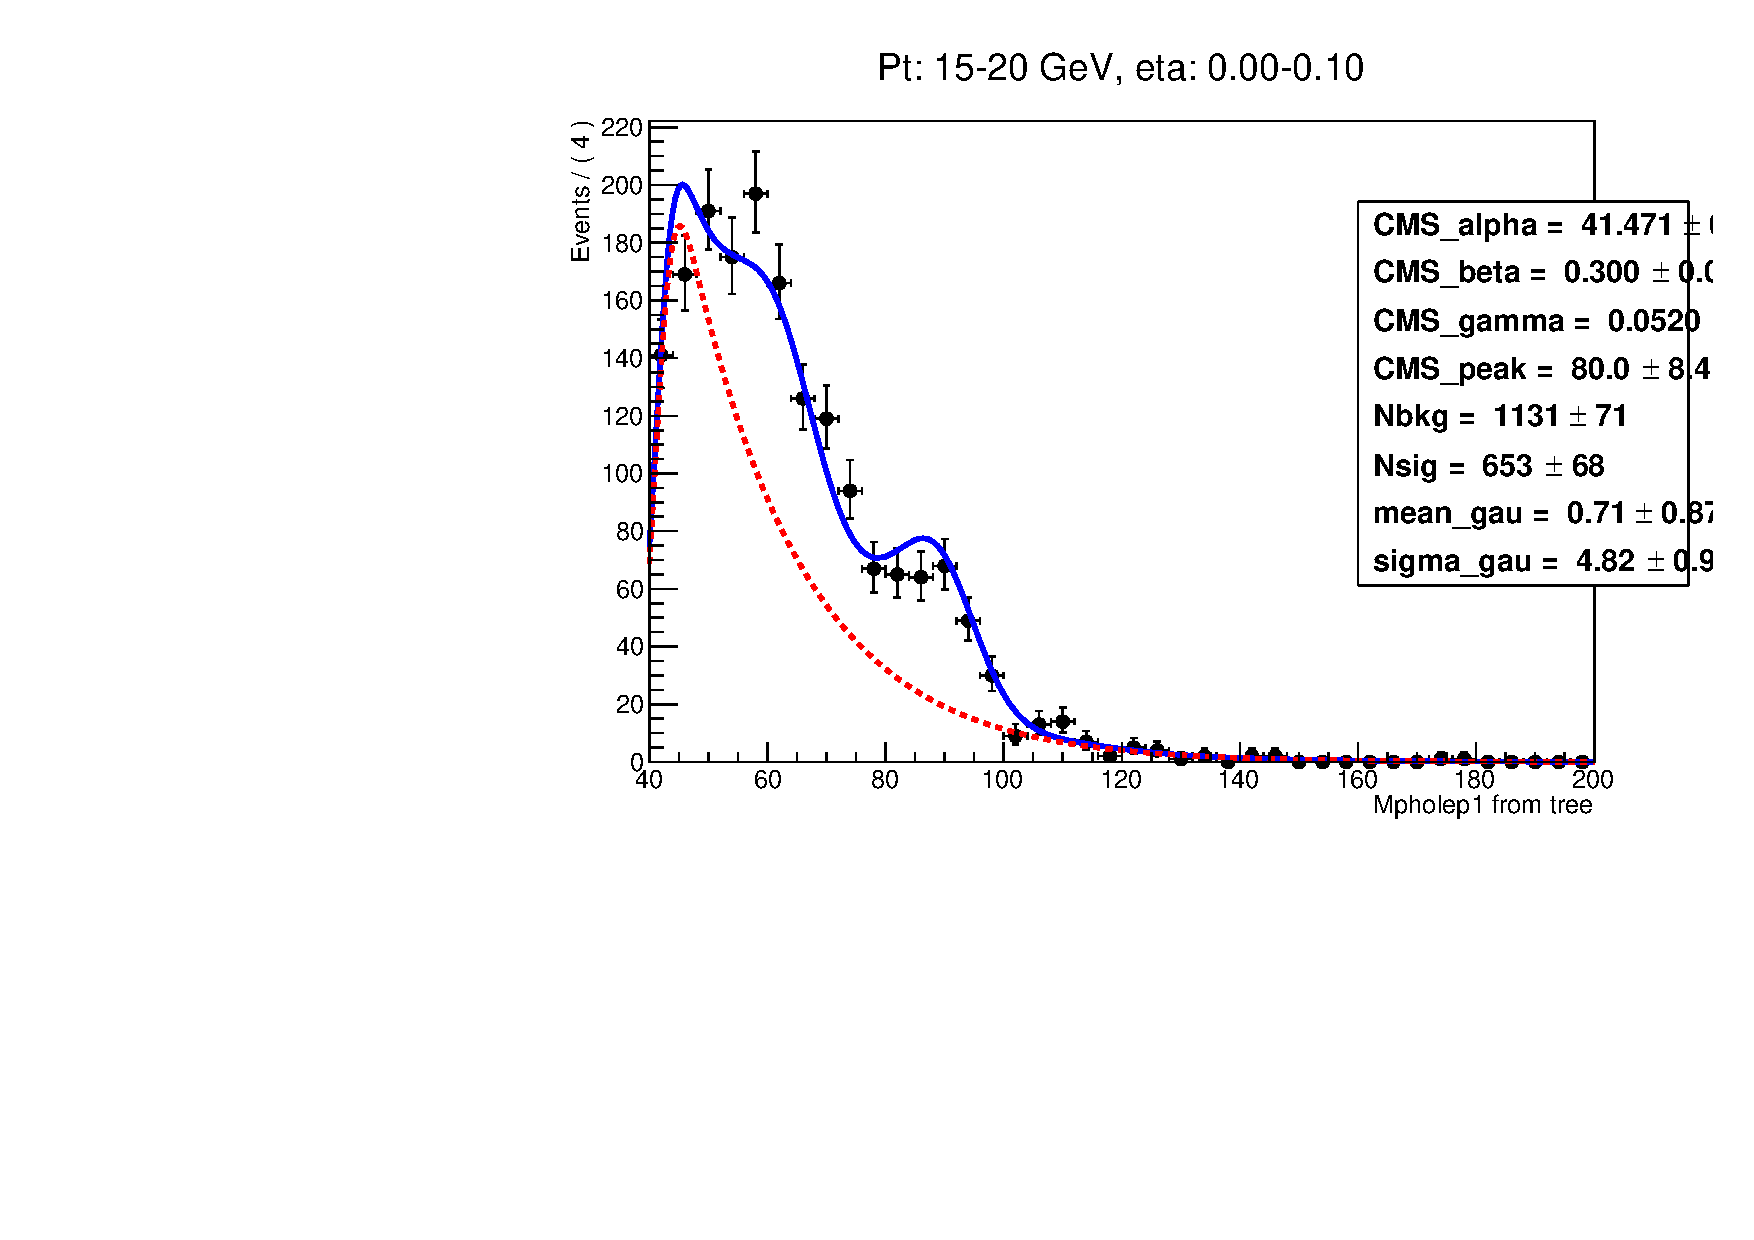
\includegraphics[width=0.45\textwidth]{../figs/figs_v11/ELECTRON_WGamma/EtoGammaFits/sa_hZmass_h_Data_EtoGamma_Enr_BARREL_pt15to20_ieta0.pdf}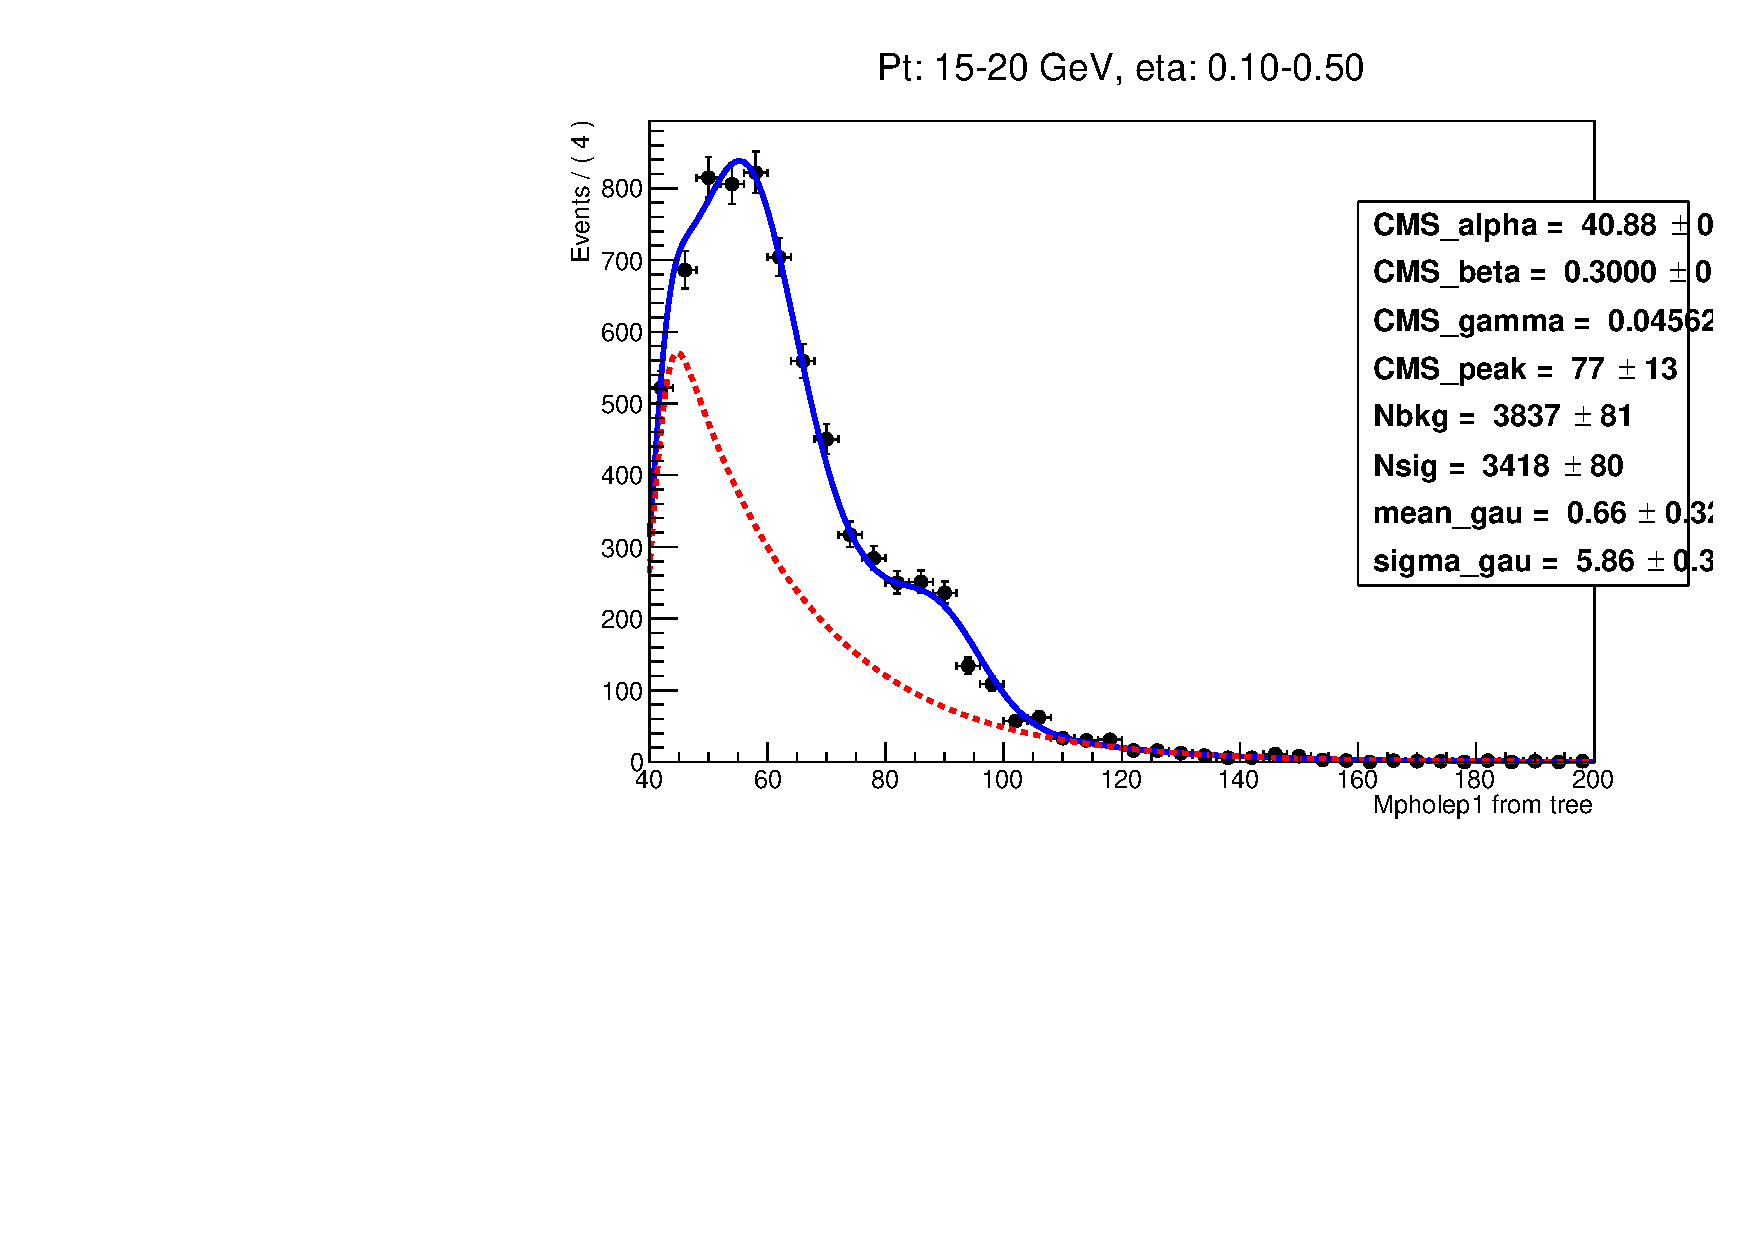
\includegraphics[width=0.45\textwidth]{../figs/figs_v11/ELECTRON_WGamma/EtoGammaFits/sa_hZmass_h_Data_EtoGamma_Enr_BARREL_pt15to20_ieta1.pdf}\\
   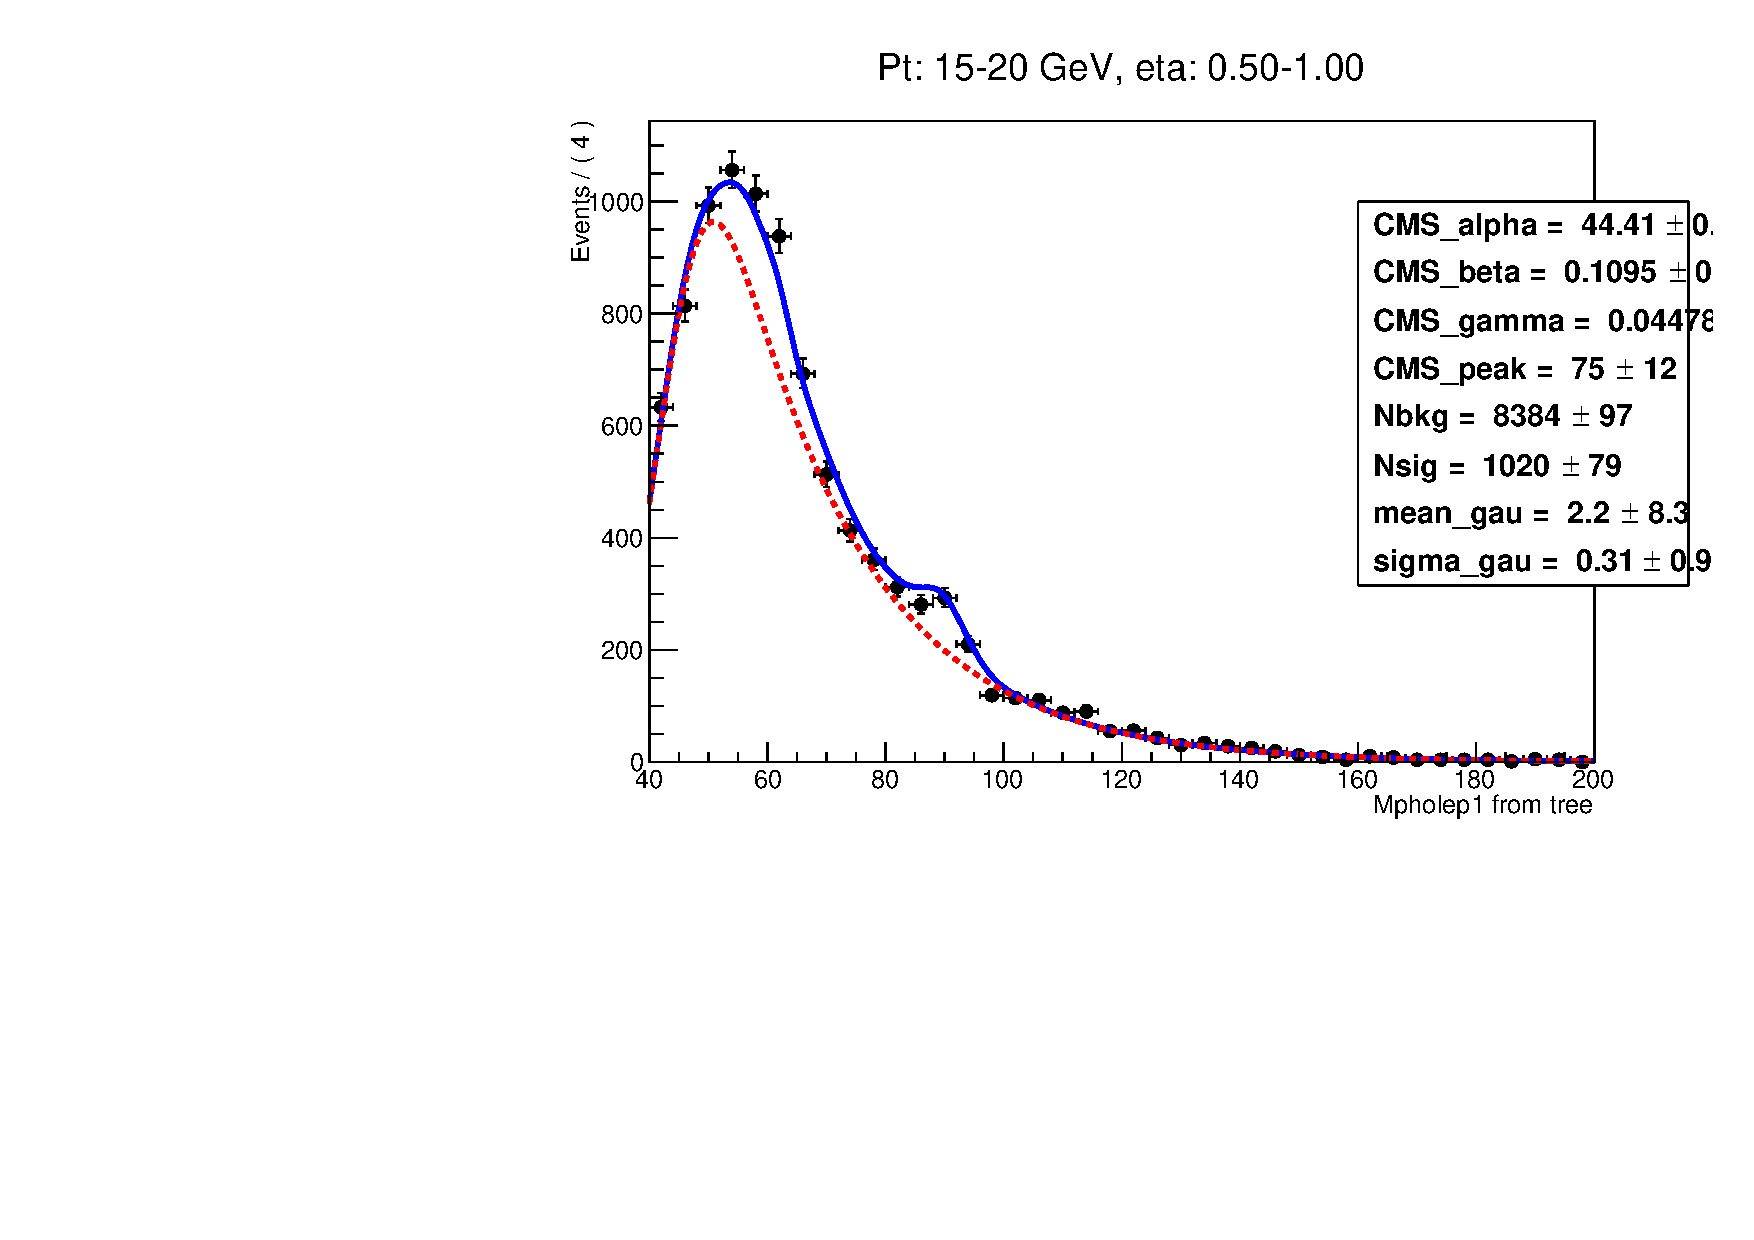
\includegraphics[width=0.45\textwidth]{../figs/figs_v11/ELECTRON_WGamma/EtoGammaFits/sa_hZmass_h_Data_EtoGamma_Enr_BARREL_pt15to20_ieta2.pdf}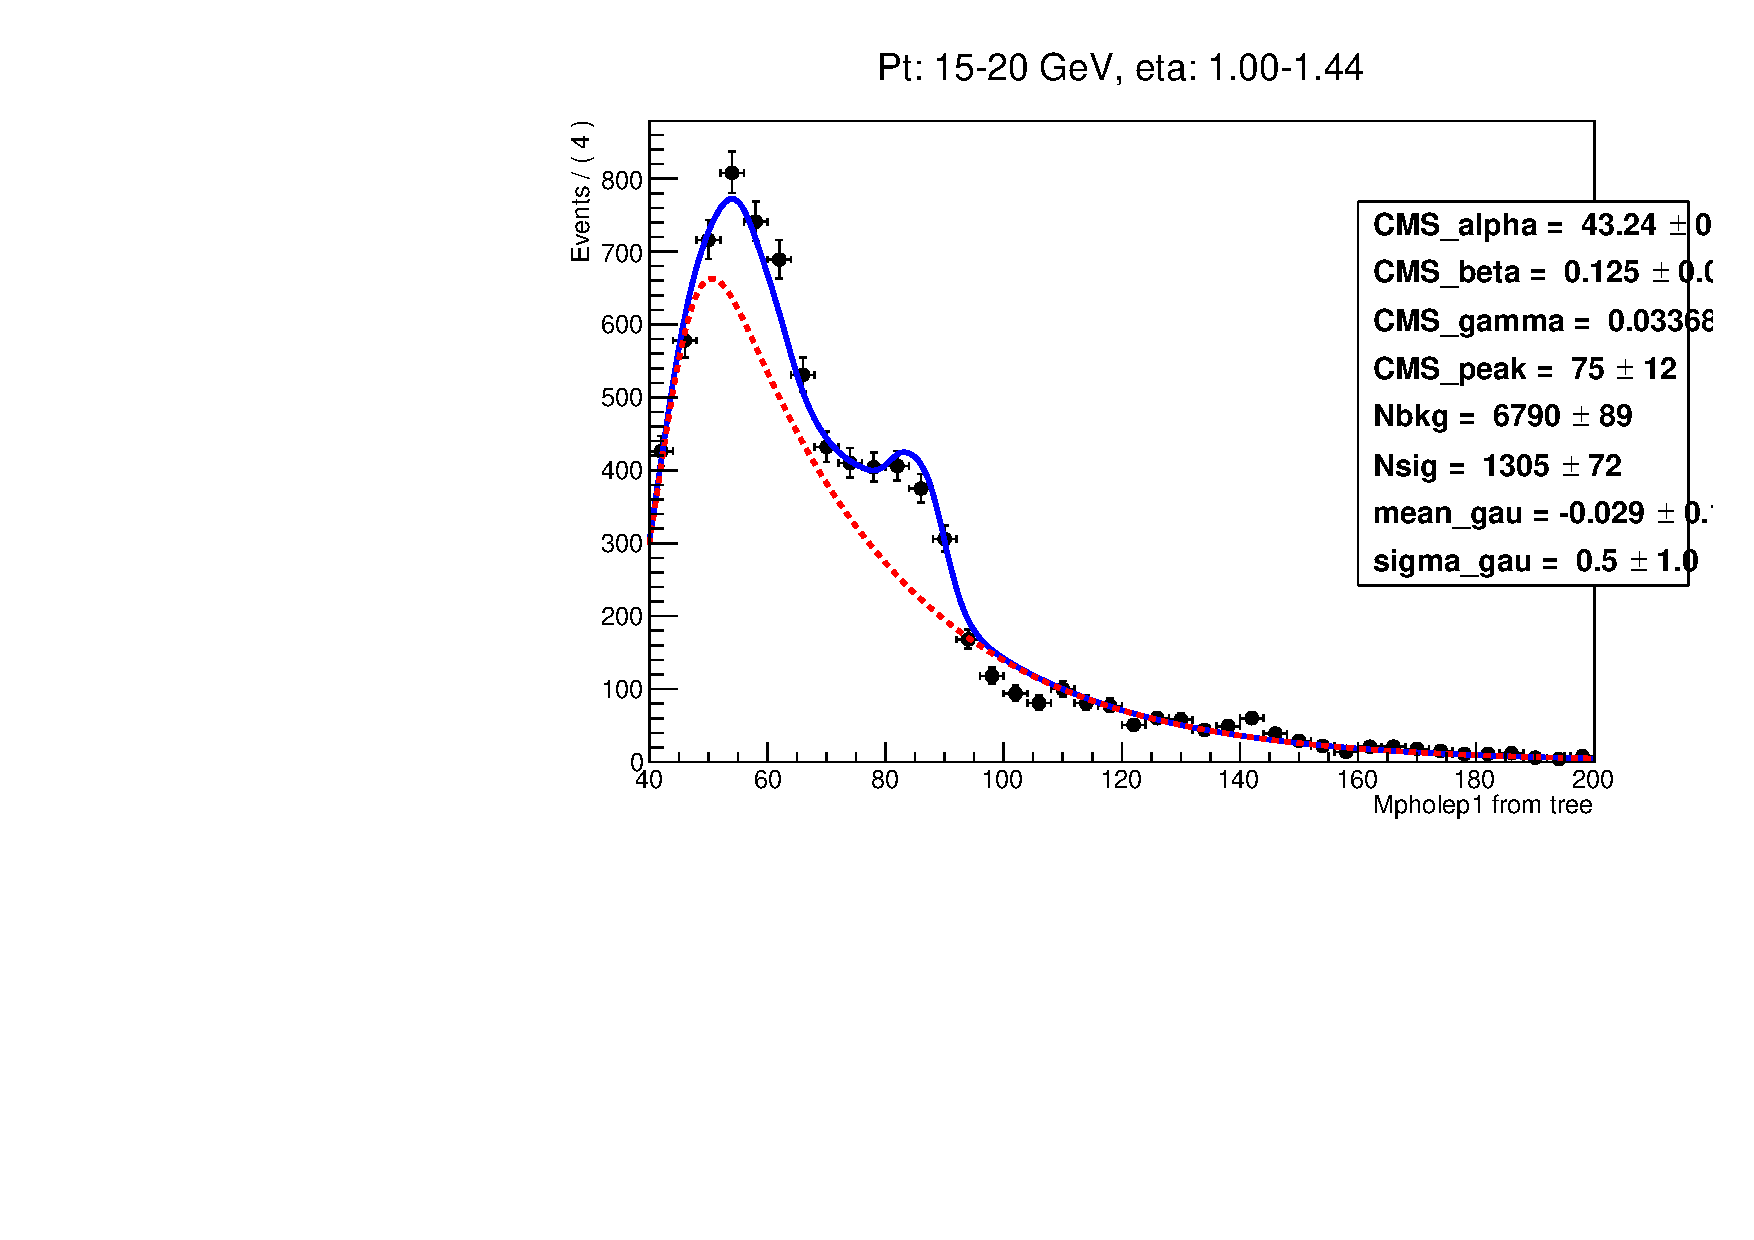
\includegraphics[width=0.45\textwidth]{../figs/figs_v11/ELECTRON_WGamma/EtoGammaFits/sa_hZmass_h_Data_EtoGamma_Enr_BARREL_pt15to20_ieta3.pdf}\\
  \caption{$M_{e,\gamma}$ fits, W$\gamma$, electron channel, 15-20 GeV, barrel, 4 eta bins}
  \end{center}
\end{figure}
\end{frame}%\frametitle{$M_{e,\gamma}$ Fit Plots. 15-20 GeV, barrel}

\begin{frame}\frametitle{$M_{e,\gamma}$ Fit Plots. 15-20 GeV, endcap}
\begin{figure}[htb]
  \begin{center}
   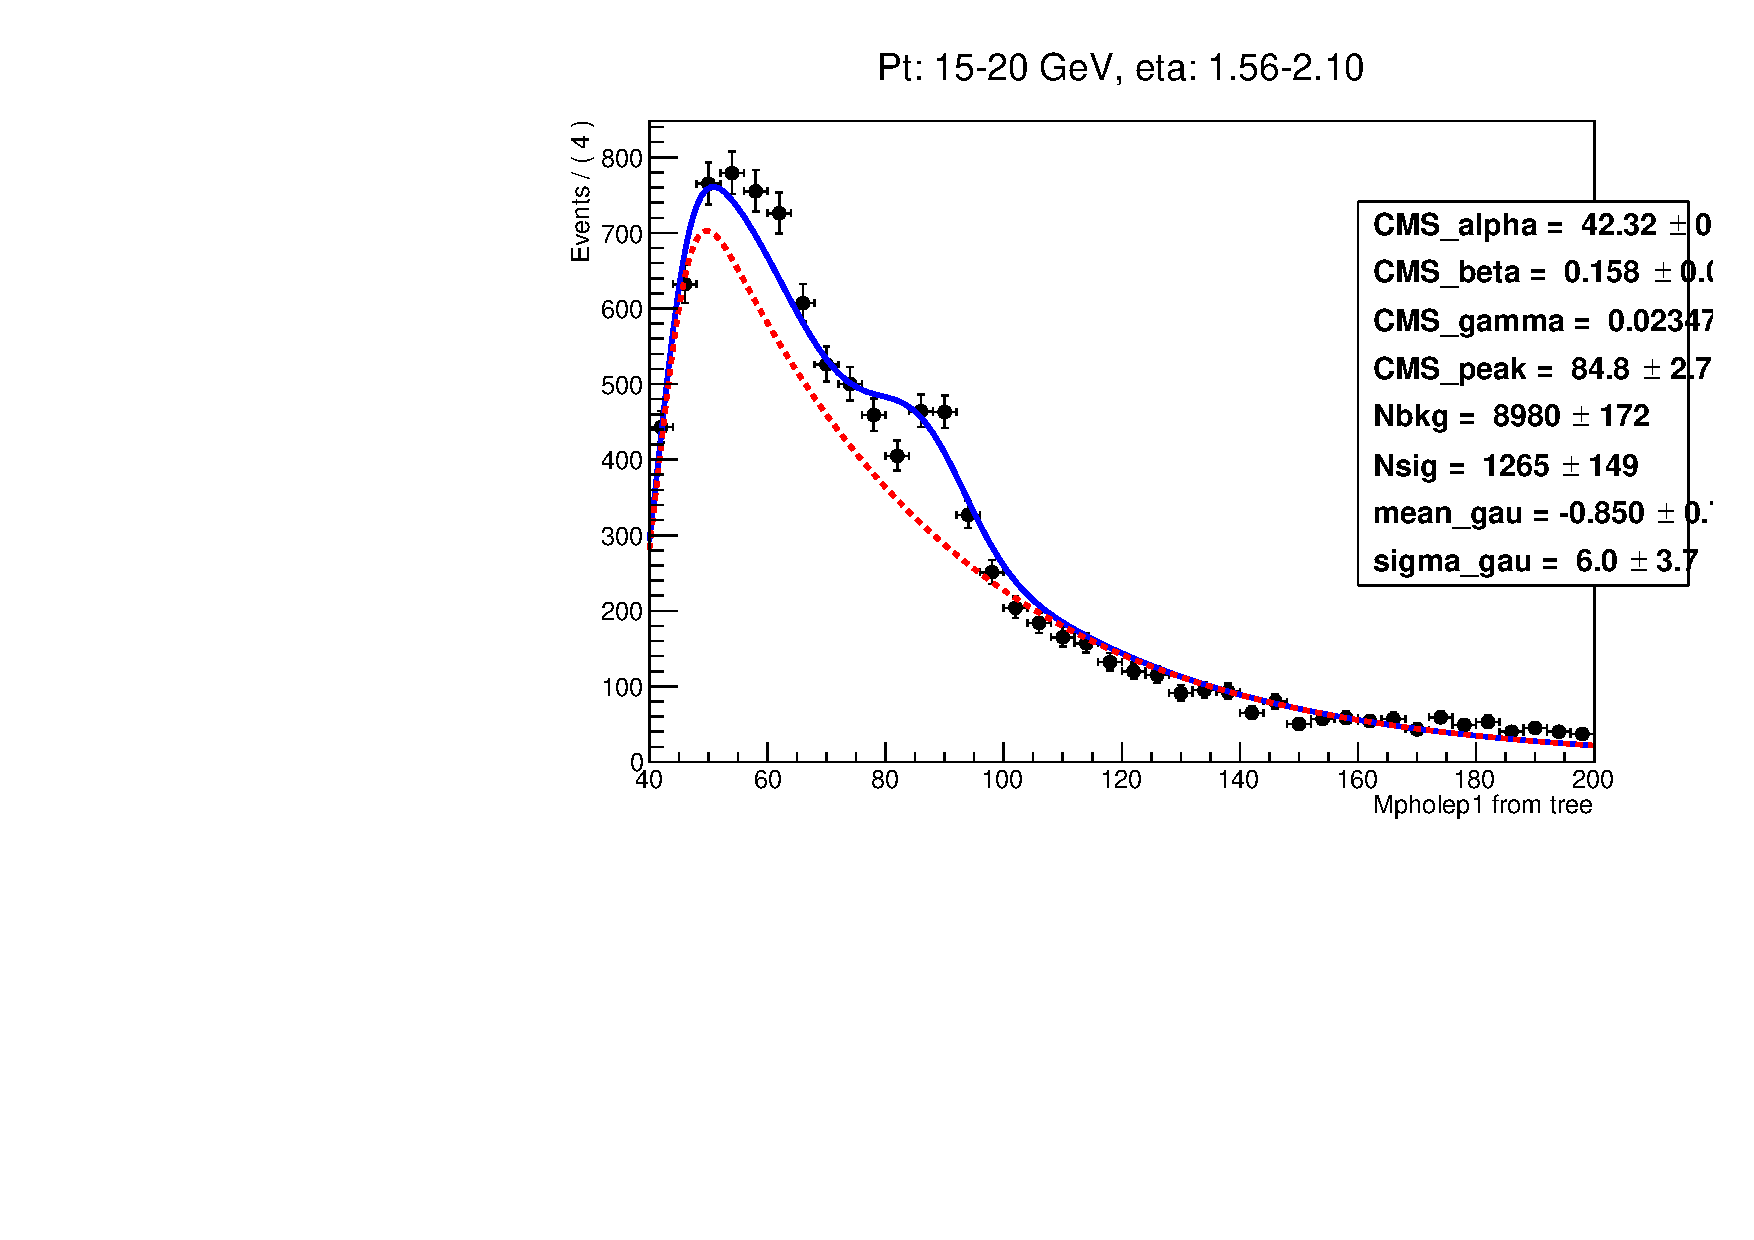
\includegraphics[width=0.45\textwidth]{../figs/figs_v11/ELECTRON_WGamma/EtoGammaFits/sa_hZmass_h_Data_EtoGamma_Enr_ENDCAP_pt15to20_ieta0.pdf}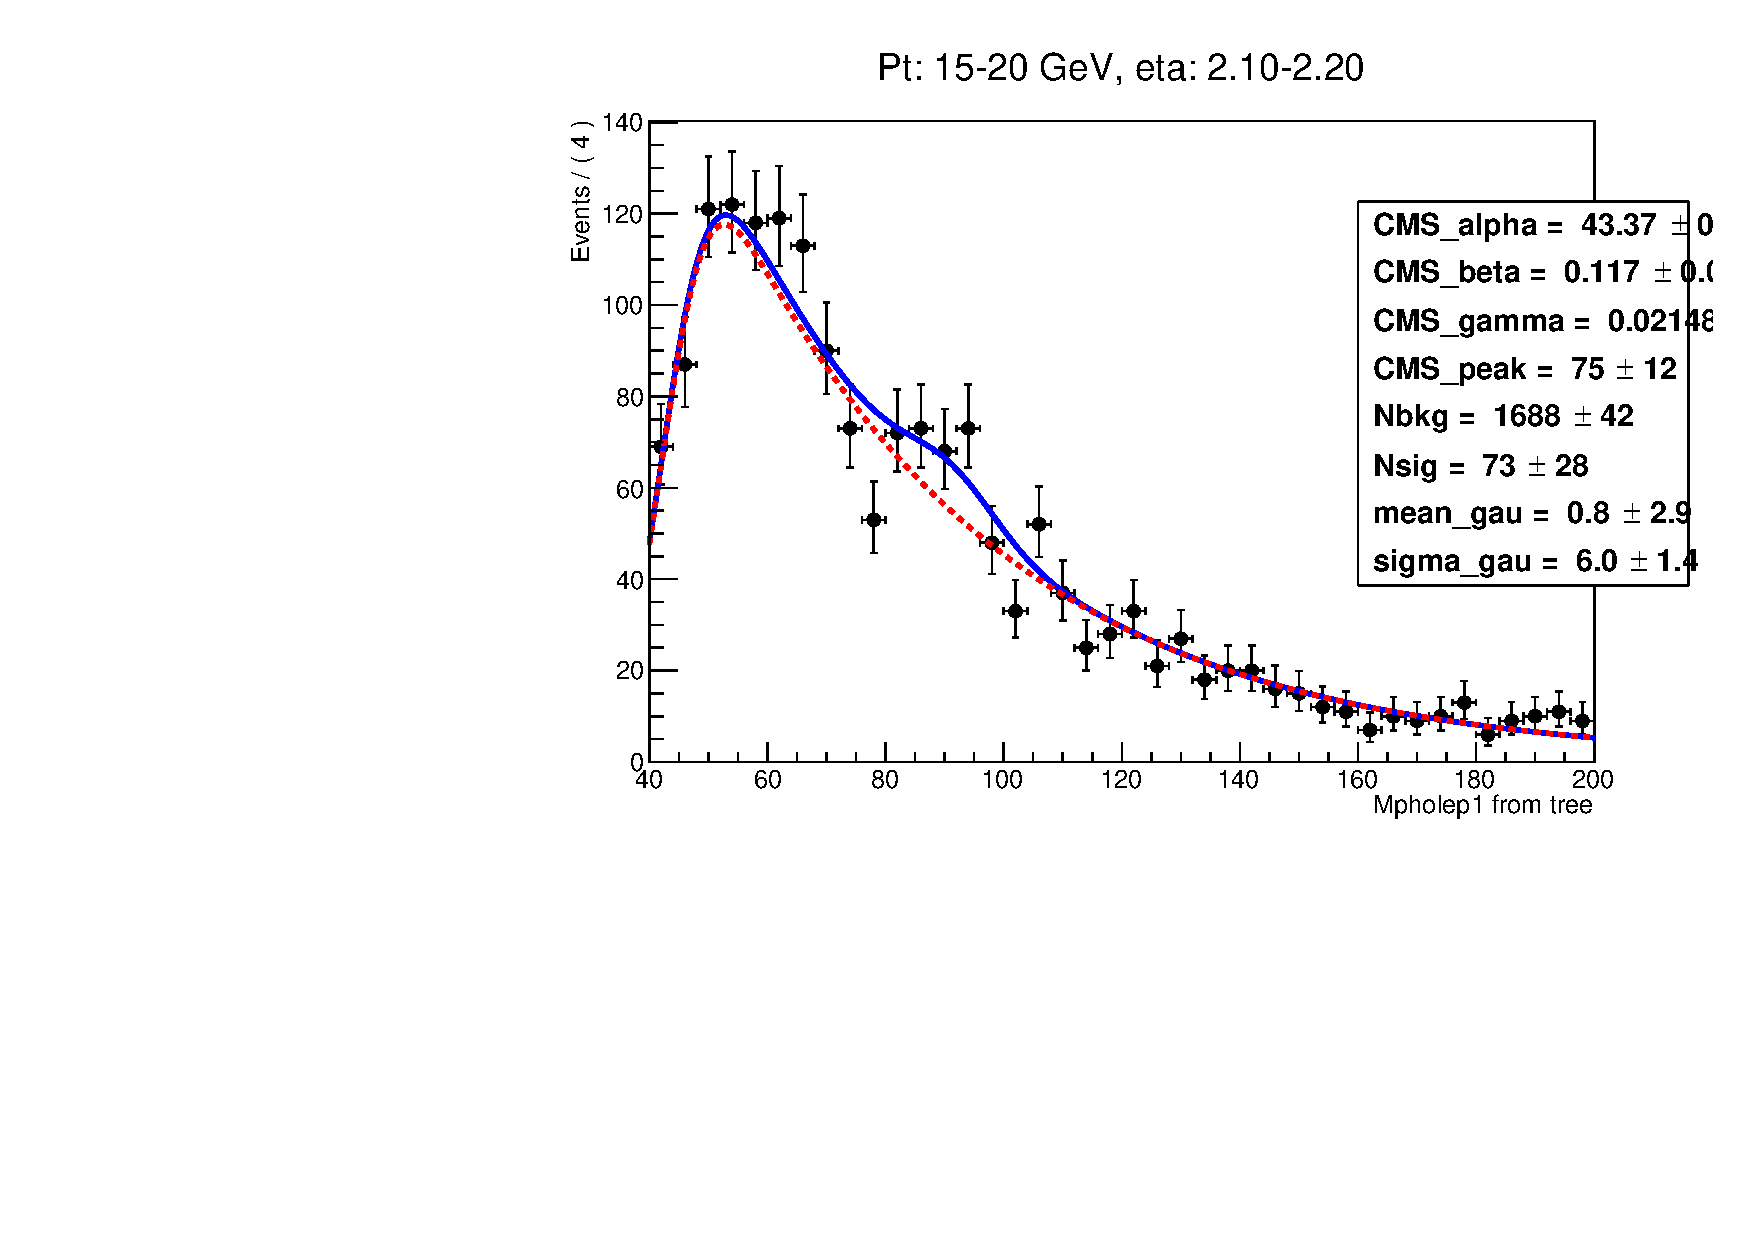
\includegraphics[width=0.45\textwidth]{../figs/figs_v11/ELECTRON_WGamma/EtoGammaFits/sa_hZmass_h_Data_EtoGamma_Enr_ENDCAP_pt15to20_ieta1.pdf}\\
   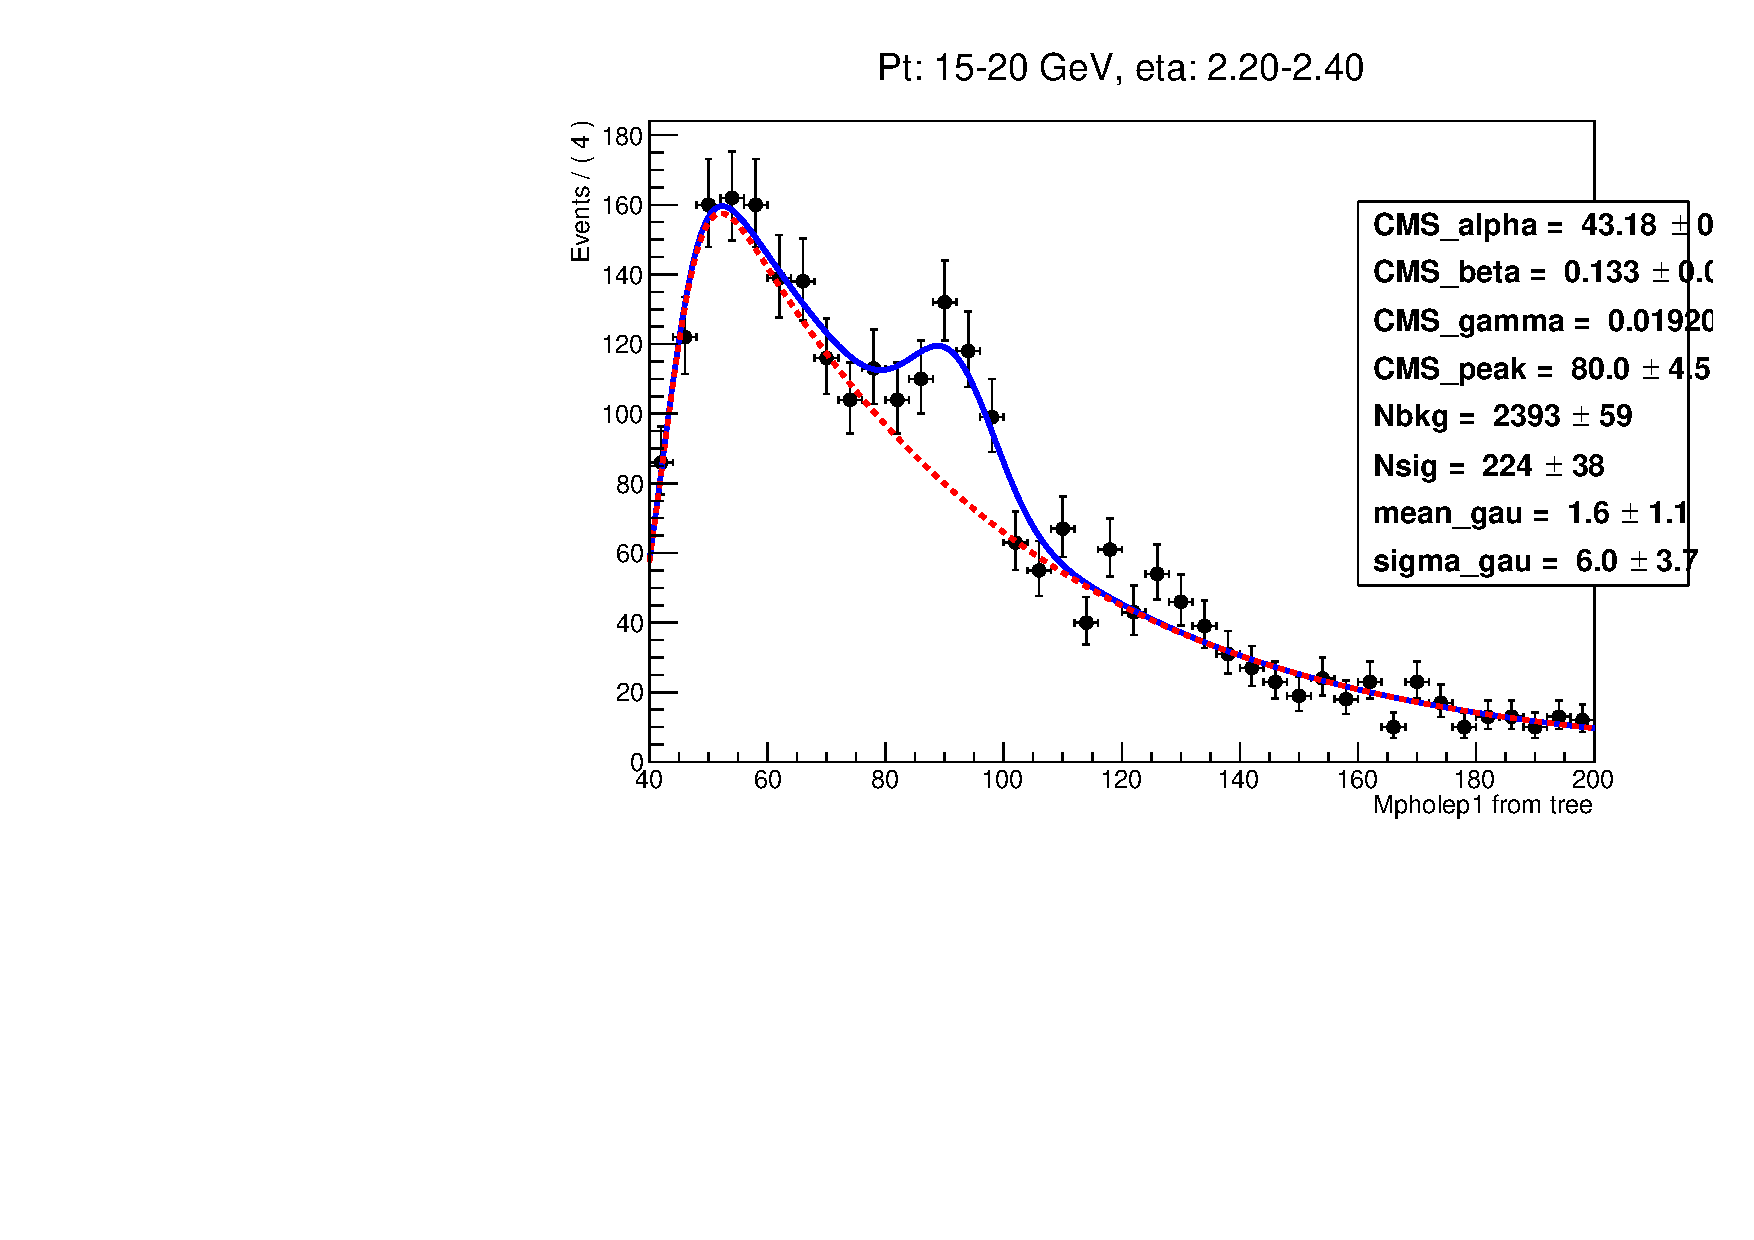
\includegraphics[width=0.45\textwidth]{../figs/figs_v11/ELECTRON_WGamma/EtoGammaFits/sa_hZmass_h_Data_EtoGamma_Enr_ENDCAP_pt15to20_ieta2.pdf}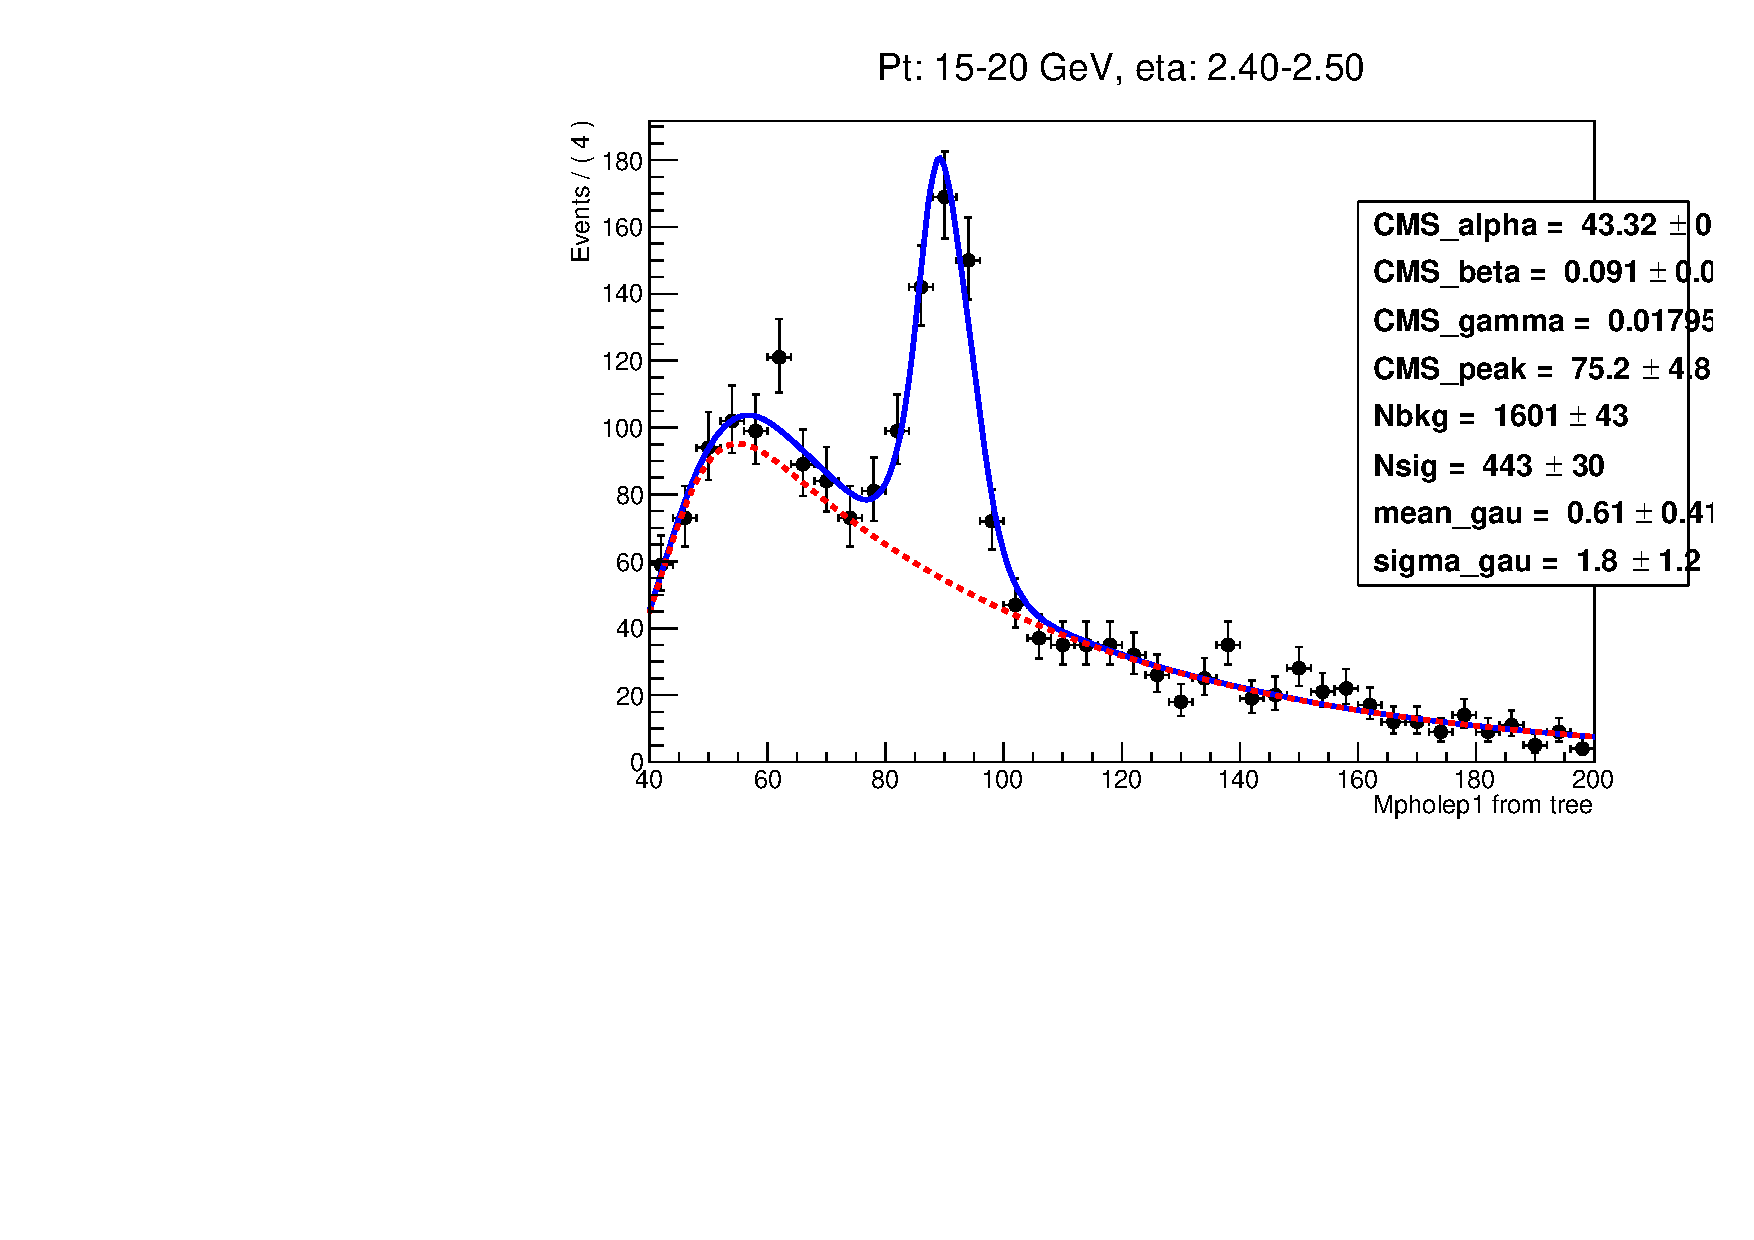
\includegraphics[width=0.45\textwidth]{../figs/figs_v11/ELECTRON_WGamma/EtoGammaFits/sa_hZmass_h_Data_EtoGamma_Enr_ENDCAP_pt15to20_ieta3.pdf}\\
  \label{fig:etogFits_15to20}
  \caption{$M_{e,\gamma}$ fits, W$\gamma$, electron channel, 15-20 GeV, endcap, 4 eta bins}
  \end{center}
\end{figure}
\end{frame}%\frametitle{$M_{e,\gamma}$ Fit Plots. 15-20 GeV, endcap}
